\documentclass[dvisvgm]{standalone}
\usepackage{amsmath}
\usepackage{amssymb}
\usepackage{amsfonts}
\usepackage{amsthm}
\usepackage{kotex}
\usepackage{tikz}
\usepackage{tkz-euclide}
\usepackage{pgfplots}
\usepackage{tikz-3dplot}
\pgfplotsset{compat=1.9}
\thispagestyle{empty}
\begin{document}

    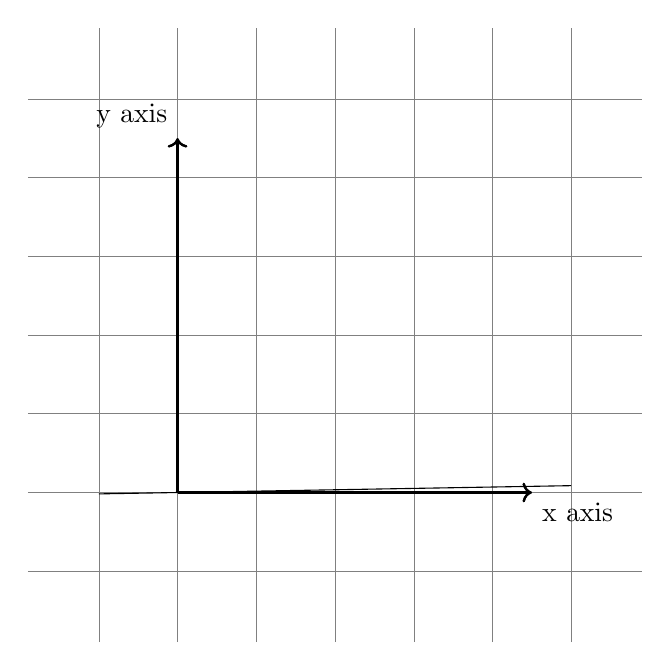
\begin{tikzpicture}
    \draw[step=1cm,gray,very thin] (-1.9,-1.9) grid (5.9,5.9);
    \draw[thick,->] (0,0) -- (4.5,0);
    \draw[thick,->] (0,0) -- (0,4.5);
    \draw[thick,->] (0,0) -- (4.5,0) node[anchor=north west] {x axis};
    \draw[thick,->] (0,0) -- (0,4.5) node[anchor=south east] {y axis};
    \draw[domain=-1:5, samples=100] plot(\x,{sin(\x)} );
  \end{tikzpicture}

\end{document}
